\documentclass[a4paper, 11pt]{article}
% TeX-template
% Copyright (c) 2024 Joseph Tooby-Smith. All rights reserved.
% Released under Apache 2.0 license.
% Paper content: 
% Copyright (c) 2024 Joseph Tooby-Smith. All rights reserved.
\usepackage{xcolor}
\usepackage{setspace}

\onehalfspacing%
%\setstretch{3} % Custom separation of lines.
\renewcommand{\arraystretch}{1.5}
%%%%%%%%%%%%%%%%%%%%%%%%%%%%%%%%
%Hyperlinks
\usepackage{hyperref}
\definecolor{mycolor}{RGB}{0,88,204}
\hypersetup{
  colorlinks=true,
  linkcolor=mycolor,
  urlcolor=mycolor,
  citecolor=mycolor
}
%%%%%%%%%%%%%
%Watermark
\usepackage{draftwatermark}
\SetWatermarkText{\color{mycolor} DRAFT}
\SetWatermarkScale{1.5}
%%%%%%%%%%%%%%%%%%%%%%%%%%%%%%%%
%Mathematics
\usepackage{amsmath}
%%%%%%%%%%%%%%%%%%%%%%%%%%%%%%%%
%Margins
\usepackage{geometry}

\geometry{
  top=0.8in,
  bottom=0.8in,
  left=1in,
  right=1in
}
%%%%%%%%%%%%%%%%%%%%%%%%%%%%%%%%
%Page numbers
\usepackage{fancyhdr}


\pagestyle{fancy}
\fancyhf{}
\fancyhead[R]{\thepage}
\renewcommand{\headrulewidth}{0pt}
\setlength{\headheight}{13.6pt}
%For the title page
\fancypagestyle{plain}{%
  \fancyhf{}
  \fancyhead[R]{\thepage}
  \renewcommand{\headrulewidth}{0pt}
}
%%%%%%%%%%%%%%%%%%%%%%%%%%%%%%%%
%Fonts

\usepackage{mathptmx}

%%%%%%%%%%%%%%%%%%%%%%%%%%%%%%%%
%Section style

\usepackage{titlesec}

\titleformat{\section}
  {\normalfont\large\centering}{\thesection.}{1em}{\MakeUppercase}
\titleformat{\subsection}
  {\normalfont\centering}{\thesubsection.}{1em}{\MakeUppercase}

  \titlespacing{\paragraph}{10pt}{0pt}{6pt}[0pt]
%%%%%%%%%%%%%%%%%%%%%%%%%%%%%%%%
%Comments

\newcommand{\js}[1]{ {\color{magenta} js:  #1}}

%%%%%%%%%%%%%%%%%%%%%%%%%%%%%%%%
%SVG images
\usepackage{svg}
%%%%%%%%%%%%%%%%%%%%%%%%%%%%%%%%
%Paragraph markers
%\newcommand{\paragraphMarker}[1]{ %{\color{gray} $\langle$#1$\rangle$}
%}
%%%%%%%%%%%%%%%%%%%%%%%%%%%%%%%
%Lean formating
\usepackage{listings}
\usepackage[T1]{fontenc}
\usepackage[utf8]{inputenc}
\usepackage{amssymb}
\usepackage{chngcntr}
\definecolor{keywordcolor}{rgb}{0.7, 0.1, 0.1}   % red
\definecolor{tacticcolor}{rgb}{0.0, 0.1, 0.6}    % blue
\definecolor{commentcolor}{rgb}{0.4, 0.4, 0.4}   % grey
\definecolor{symbolcolor}{rgb}{0.0, 0.1, 0.6}    % blue
\definecolor{sortcolor}{rgb}{0.1, 0.5, 0.1}      % green
\definecolor{attributecolor}{rgb}{0.7, 0.1, 0.1} % red

\def\lstlanguagefiles{lstlean.tex}
\lstset{
 	frame = lrtb,
 	rulecolor=\color{mycolor},
	language=lean,
	aboveskip = 5mm,
	belowskip = 5mm,
	captionpos=t
	}

\lstnewenvironment{code}[1][]%
{
   \noindent\newline
   \minipage{\linewidth}
   \vspace{0.5\baselineskip}
   \lstset{
 	frame = lrtb,
 	rulecolor=\color{mycolor},
 	escapeinside={/*!}{!*/},
	language=lean,
	aboveskip = 5mm,
	belowskip = 5mm,
	xleftmargin=2mm,
	xrightmargin=2mm,
	}
	}
{\endminipage\newline}
\lstnewenvironment{codeLong}[1][]%
{
   \lstset{
 	frame = lrtb,
 	rulecolor=\color{mycolor},
 	escapeinside={/*!}{!*/},
	language=lean,
	aboveskip = 5mm,
	belowskip = 5mm,
	xleftmargin=2mm,
	xrightmargin=2mm,
	}
	}
{}
%%%%%%%%%%%%%%%%%%%%%%%%%%%%%%%%
%Links in code block
% put at top of code block using
% /*!\codeLink{...}!*/
\newcommand{\codeLink}[1]{
  \vspace{-0.5cm}\hfill\href{https://github.com/HEPLean/HepLean/blob/1b951994ae3d882242b02d23957ef1ee7fa05f3d/HepLean/#1}{(source)}
  }
  \newcommand{\codeBreakdownLink}[2]{
  \vspace{-0.5cm}\hfill\href{https://github.com/HEPLean/HepLean/blob/1b951994ae3d882242b02d23957ef1ee7fa05f3d/HepLean/#1}{(source)}
  (breakdown \ref{#2})
  }
 \newcommand{\textLink}[1]{\href{https://github.com/HEPLean/HepLean/blob/1b951994ae3d882242b02d23957ef1ee7fa05f3d/HepLean/#1}{source}}
 \newcommand{\textLinkB}[1]{\href{https://github.com/HEPLean/HepLean/blob/1b951994ae3d882242b02d23957ef1ee7fa05f3d/HepLean/#1}{(source)}}
%%%%%%%%%%%%%%%%%%%%%%%%%%%%%%%%
%Title, author, date
\title{Index notation in Lean 4}
\author{Joseph Tooby-Smith \\ \textit{Reykjavik University}}
\date{\today}
%%%%%%%%%%%%%%%%%%%%%%%%%%%%%%%%

\begin{document}
\counterwithin{lstlisting}{section}
\maketitle
\vspace{-1cm}
\begin{abstract}
Index notation is a tool commonly used in physics to manipulate tensors.
In physics, we use index notation for three different types of tensors: 
Einstein tensors (e.g., ordinary vectors and matrices), Lorentz tensors, and 
Van der Waerden tensors. In this paper, we discuss how these are implemented in Lean 4 using a 
general mathematical theory based on category theory, and related to the notation of an operad.
\end{abstract}

\section{Introduction}

A previous work by the current author, presented the first steps of digitalizing (or formalizing)
results from high energy physics into the interactive theorem prover Lean 4. This 
project is called HepLean. Lean is a programming language whose syntax looks similar to 
what we pen-and-paper mathematics, and is used to write and automatically check 
 statements of definitions and theorems, and proofs of theorems.
HepLean has four main motivations: \js{sorry}


When writing and proving results on paper, the physicists is accustumed to using notation, and no
notation abounds in physics more than index notation.
Thus as part of the larger HepLean project, index notation has been implemented by 
the author in to Lean 4.
Any such implementation must satisfy two basic requirements: 
\begin{enumerate}
  \item Must be mathematically rigourous. 
  \item Must be easy to use.
\end{enumerate} 
The first requirement is a consequence of Lean being a proof assistant, and not able to accept 
anything else but formally defined results. 
The second requirement is due to the fact that many other results will depend on the 
implementation of index notation. We beleive the implementation dicussed within this paper 
does satisfy both of these requirements.  



\begin{itemize}
\item Notational conventions abound in physics, and non-more so then index notation. 
\item Notation, in general, is a way for the writer to compactly write down a term in a 
  mathematical expression. The reader can implicitly unfold or elborate the compactly written term 
  back into its full underlying meaning. 
\item Index notation is a compact way of writing expressions involving tensors.
\item With tensors there is a notion of contraction, evaluation and permutation.
\item All of these notions can defined independently of index notation.
\item Index notation is a way of writing these operations in a compact way.
\item In a previous work by the current author, the first foray of formalizing high energy physics 
  in Lean 4 was undertaken, in a project called `HepLean'.
\item One aim of that project is to make Lean easier for the high-energy phsycisists to use. 
\item Motiviated by this aim, we have implemented index notation in Lean 4.
\item In this paper, we will discuss how this is done.
\item This is, of course, not the first paper dicussing the implmentation of index notation in a 
  programming language. However, Lean, being a proof assistant, has a different set of requirements. 
\item In particular, Lean has to be provided a proof of everything. 
\item We also believe that the underlying mathematics used to implement index notation here 
 is novel. 
\end{itemize}

\section{Implementation of index notation into Lean 4}
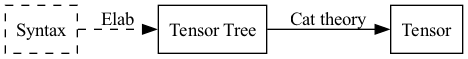
\includegraphics[width=\textwidth]{overviewFlow.png}
\begin{itemize}
  \item In this paper we will discuss each part of this diagram from the left to the right.
\end{itemize}
\subsection{Defining tensors}

\subsubsection{Building blocks of tensors and color}

\begin{itemize}
\item Tensors are built from a set of representations.
\item For example, complex Lorentz tensors are built from six representations of the group $SL(2, \mathbb{C})$.
\item To each of these building blocks we assign a label, which we call the color.
\item For complex complex Lorentz tensor the colors are. 
\item In Lean this information is encoded as follows. We define a type $C$ containing the colors.
\item For complex Lorentz tensors this type is \js{sorry} 
\item Then we define a discrete functor from $C$ to the category of complex representations of $SL(2, \mathbb{C})$.
\item For complex Lorentz tensors this functor is defined as \js{sorry}.
\item We will see a number of reasons shortly why we have used a functor here. 
\end{itemize}

\subsubsection{A general tensor}

\begin{itemize} 
\item A general tensor of a given species is roughly an element of a vector space 
  built by taking the tensor product of the building block representations. 
\item To be more formal, let $X$ be a type, and $f : X \to C$ a function from that type 
  into the type of colors. 
  Associated with $f$ we can define a representation of $SL(2, \mathbb{C})$, 
  by taking the tensor product of the representations $f(x)$ for $x \in X$. 
\item A general complex Lorentz tensor is then an element of one of these representations.
\item To give an explicit example $X$ may be something like $Fin 2$, i.e. the type of 
  numbers $(0,1)$. The function $f$ may be $![Color.up, Color.down]$, and the corresponding 
  representation is then (equivalent to) \js{sorry}. 
\item This can can be described categorically. 
\item The functions $f :X \to C$ live in a category whose objects are \js{sorry} and 
 whose morphisms are \js{sorry}. This is equivalent the core of \js{sorry}. 
\item As such, we denote this category $\mathcal{S}_{/C}^\times$.
\item This category has a symmetric monoidal structure, given by the disjoint union of $X$.
\item There is a functor $C \to \mathrm{Rep}_{SL(2, \mathbb{C})} \to 
  \mathrm{BraiFun} \mathcal{S}_{/C}^\times \mathrm{Rep}_{SL(2, \mathbb{C})}$.
  from functors from $C \to \mathrm{Rep}_{SL(2, \mathbb{C})} $ to symmetric 
  monoidal \js{sorry}.
\item We call this functor $\mathrm{lift}$. 
\item A general tensor of a given species, which has discrete functor $F_{dis}$ is then 
 an element of a representation in the image of $\mathrm{lift}\; F_{dis}$.
\item We will be most intrested in the case when $X = Fin n$ for some $n$.
\end{itemize}

\subsubsection{Basic operations}

\begin{itemize} 
\item The formalisim we have discribed thus far gives us basic oprations on tensors for free.
\item We get addition, scalar multiplication and the action of the group $SL(2, \mathbb{C})$ from 
  the fact that things sit in representations. 
\item We also get the tensor product of two tensors, from the category of representations 
  and the fact that our lift function is symmetric monoidal. 
\item We get permutation of indices from the fact we have a functor. 
\item We get negation of tensors because \js{sorry}
\item We also get the interplay between all of these
\item There somethings we do not get for free however: Contraction, the unit of the contraction, 
  and the metrics. 
\item To define these we need introduce an involution $\tau : C \to C$. We will call the image of 
  $c$ under $\tau$ the dual of $c$.
\item Colors can be self-dual, as there for Einstein tensors, for which there is only one color. 
\item From $\tau$ we get a functor $\tau_* : \mathcal{S}_{/C}^\times \to \mathcal{S}_{/C}^\times$.
\item We let $F_\tau$ be the functor from $C$ to $F(c) \otimes F(\tau c)$.
\item To define contraction we define a natural transformation $ F_\tau \to \mathbb{1}$.
\item That is for each $c$ a morphism of representations from   $F(c) \otimes F(\tau c)$ to the 
  trivial representation.
\item To give an example for complex Lorentz tensors \js{sorry}
\item Using $F_\tau$ we can contract indices of tensors of dual colors. 
\item Lifiting $F_\tau$ gives us a functor which would allow us to contract all indices of a tensor
 at ones. This may be useful for come computations. 
\item In addition to contraction we want the notion of a metric.  
\item \js{Unit}
\item  \js{Conditions}
\end{itemize}

\subsubsection{Tensor Species}

\begin{itemize}
  \item The data we have given so far consitutes what we have losely being calling a Tensor species. 
  \item In Lean we make this more precise 
\end{itemize}

\subsection{Tensor trees}
\subsubsection{Structure}
\begin{itemize}
  \item A tensor expression consists of a series of tensors and operations performed on them. 
  \item We can represent such an expression using a tensor tree, similar to the notion of a 
    syntax tree.
  \item A tensor tree has different types of nodes either representing a tensor or a operation 
    on or between tensors. 
  \item Since we really only care about tensors with $X = Fin n$, tensor trees in Lean are 
    implemented only for these. 
  \item Let us give the definition of a tensor tree and then dicuss in turn each of the nodes. 
  \item \js{Lean defn of tensor tree}
  \item The basic node is a tensor node. The definition in Lean tells us how this is defined. 
  \item Then for each operation addition, scalar mult, group action etc. we get a node. 
  \item For example let us look at contraction 
  \item \js{sorry}
  \item How we turn these tensor trees into tensors will be dicussed in the next section
\end{itemize}

\subsubsection{To a tensor}

\begin{itemize}
  \item The notion of a tensor tree is defined without reference to the category theory 
    we have been discussing. 
  \item We can however turn a tensor tree into a tensor using said constructions. 
  \item The definition of how we do this is defined recursively. 
\end{itemize}

\subsubsection{Using Tensor trees in proofs}
\begin{itemize}
  \item \js{Discuss fact about `tensor\_eq'}
\end{itemize}
\subsection{Elboration}
\begin{itemize}
  \item We have dicussed the implementation of tensor species into Lean, and how to write
    tensor expressions using tensor trees.
  \item Really this is all one needs to effectively. 
  \item However, we want our theorems to look like they do on paper. 
  \item This is the role of the elaborator, which here takes a string written in lean code 
    and turns it into a tensor tree.
  \item It is perhpase easist to give examples: 
  \item The basic notation for a tensor nodes is \js{sorry}. Note that ... are free indices, 
    it does not matter what we call them the expression is the same. 
  \item The product of two tensors is written as \js{sorry}.
  \item The contraction of two tensors is written as \js{sorry}. Again note that the indices 
    are free so we can call them anything without chaning how lean reads the expression. 
  \item We also define a special notation of equality and addition. which takes account of permutation.
  \item This part of the Lean code is not formally verified, it is just telling lean how to 
    read the notation. Once the tensor tree is created and we start using that, things are formally 
    verifeid.
\end{itemize}
\section{Examples}

\begin{itemize}
\item We give two examples of theorems and proves related to index notation.
\item Our first example is related to symmetric and anti-symmetric tensors. 
\item For this example we will go into explicit detail.
\item Our second example is a more detailed one, where we prove that ... 
\item For this example we will only give a sketch of the prove, and discuss how things are done.
\end{itemize}

\subsection{Example 1: Symmetric and anti-symmetric tensor}

Let  $S_{\mu \nu}$ be complex Lorentz tensors where $\mu$ and $\nu$ are 
4-vector indices. The corresponding 
\begin{code}
(S : complexLorentzTensor.F.obj (OverColor.mk ![Color.down, Color.down]))
\end{code}

To explain this notation let us work from the right to the left.

\subsection{Example 2: Contracting Pauli matrices}


\section{Future work}

\begin{itemize}
\item Informal lemmas and definitions. 
\item Improvement of tactics. 
\item spinor-hleicity formalism. 
\item Tensor fields and derivatives. 
\end{itemize}
\bibliographystyle{unsrturl}
\begin{spacing}{0.5}
\bibliography{MyBib}
\end{spacing}


%%%%%%%%%%%%%%
\end{document}
